\pdfminorversion=4
\documentclass[aspectratio=169]{beamer}
\usepackage{animate} % for animation
\usepackage{array,multirow,graphicx}
\usepackage{multicol}
\usepackage{etoolbox}
\graphicspath{{gambar/}}
\setbeamertemplate{caption}[numbered]
\setbeamertemplate{section in toc}[sections numbered]

% Hide subsubsections from TOC, but keep PDF bookmarks with beamer
\hypersetup{bookmarksopen=true,bookmarksopenlevel=4}
\setcounter{tocdepth}{4}

\renewcommand{\figurename}{Gambar.}
\renewcommand{\tablename}{Tabel.}

\usetheme[pageofpages=of,	% String used between the current page and the
							% total page count.
			alternativetitlepage=true,% Use the fancy title page.
			titleline=true,
			titlepagelogo=OK-LOGO-ITK.jpg
%          	 titlepagelogo=fig/jaist_logo.png
			]{Torino}
			% change /beamerinnerthemefancy.sty to resize the logo
\usecolortheme{freewilly}

\makeatletter
\patchcmd{\beamer@sectionintoc}{\vskip1.5em}{\vskip0em}{}{}
\makeatother

\author{Tim Dosen Pengampu \\
	Rangkaian Elektronika II}
\title{RANGKAIAN ELEKTRONIKA II}
\subtitle{Penguat Diferensial}
\institute{Teknik Elektro \\ Institut Teknologi Kalimantan \\ Balikpapan, Indonesia}
\date{\tiny Februari 22, 2021}

% The log drawn in the upper right corner.
\logo{
\includegraphics[height=0.13\paperheight]{OK-LOGO-ITK.jpg}}

\begin{document}

\begin{frame}[t,plain]
\titlepage
\end{frame}

%\begin{frame}{Bahan Kajian}
%	\begin{multicols}{2} % Two columns for outline
%    \tableofcontents[subsectionstyle=hide]
%	\end{multicols}
%\end{frame}

\section{Pengantar}
\begin{frame}{Pengantar}
	\begin{itemize}
		\item Istilah Operational amplifier (op-amp) merujuk kepada sebuah amplifier/penguat yang menjalankan suatu operasi matematika.
		\item Dalam sejarahnya, op-amp pertama digunakan di dalam komputer analog untuk melakukan operasi penjumlahan, perkalian dan lainnya.
		\item Op-amp dibuat sebagai sirkuit diskrit $ \rightarrow $ sekarang kebanyakan op-amp adalah sirkuit terintegrasi/ integrated circuits (IC). 
	\end{itemize}
\end{frame}

\begin{frame}{Pengantar}
	\begin{figure}
		\centering
		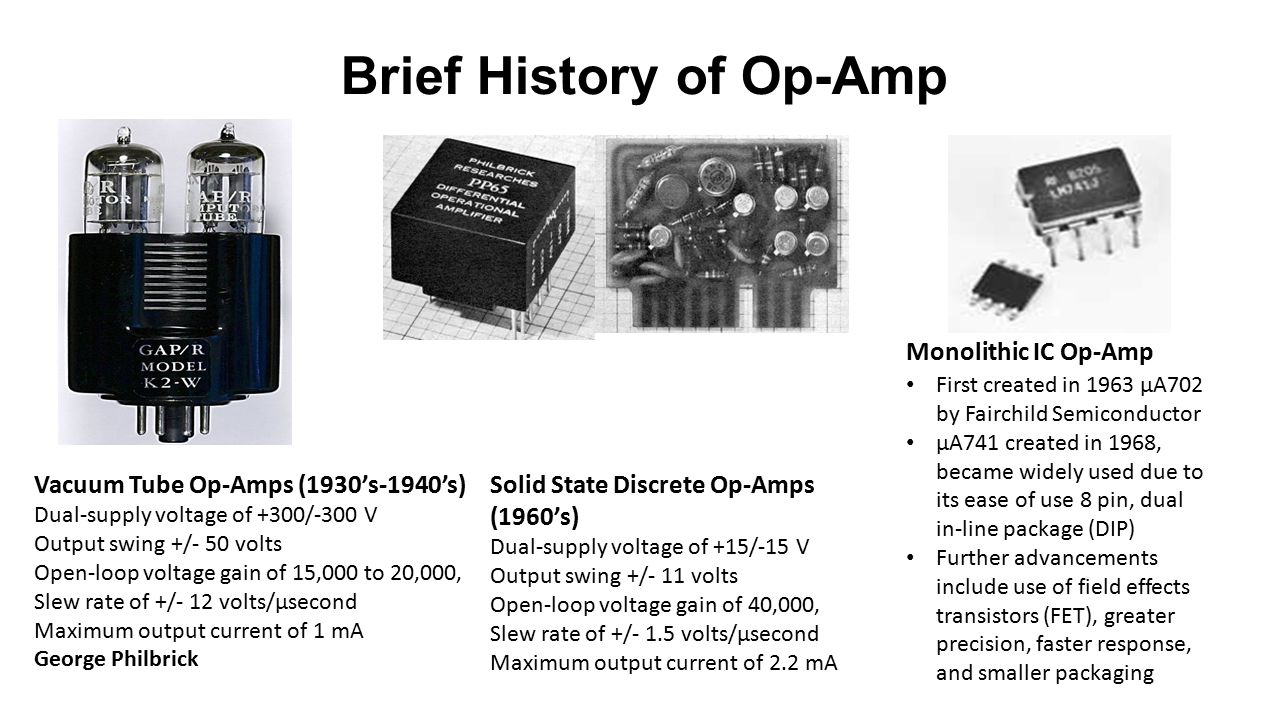
\includegraphics[height=0.75\textheight]{gambar/01.history-op-amp}
		\caption{Perkembangan op-amp}
		\label{fig:history-op-amp}
	\end{figure}
\end{frame}

\begin{frame}{Pengantar}
	\begin{itemize}
		\item Op-amp $ \rightarrow $ penguat DC/DC amplifier dengan voltage gain/penguatan tegangan yang sangat besar, impendansi input yang sangat besar, dan impedansi output yang sangat kecil.
		\item Frekuensi unity gain dari 1 hingga lebih dari 20 Mhz.
		\item IC op-amp adalah sebuah blok fungsional yang lengkap dengan pin eksternal.
		\item Hanya dengan menghubungkan pin tersebut ke suplai tegangan dan beberapa komponen, kita dapat dengan cepat membuat segala jenis rangkaian yang berguna.
	\end{itemize}
\end{frame}

\begin{frame}{Pengantar}
	\begin{itemize}
		\item Rangkaian input yang paling banyak digunakan di op-amp adalah sebuah penguat diferensial/ differential amplifier.
		\item Konfigurasi dari penguat ini memberikan banyak karakteristik input di IC.
		\item Penguat diferensial juga dapat dikonfigurasi dalam bentuk diskrit untuk digunakan dalam komunikasi, instrumentasi, dan rangkaian kontrol industri.
		\item \textbf{Kita akan fokus pada penguat diferensial yang digunakan dalam IC.}
	\end{itemize}
\end{frame}

\begin{frame}{Pengantar}
	\begin{itemize}
		\item Sub-CPMK:
		\begin{itemize}
			\item Mahasiswa mampu menganalisis rangkaian penguat diferensial (C4, P3, A3)
		\end{itemize}
		\item Bahan Kajian
		\begin{enumerate}
			\item Konsep dasar penguat diferensial;
			\item Analisis DC dari penguat diferensial;
			\item Analisis AC dari penguat diferensial;
			\item Common‐mode gain;
		\end{enumerate}
	\end{itemize}
\end{frame}

\section{Penguat Diferensial}
\begin{frame}{Penguat Diferensial}
	\begin{enumerate}
		\item Transistor, dioda, dan resistor adalah komponen-komponen praktis yang ada di dalam IC.
		\item Kapasitor mungkin dapat digunakan, tapi ukurannya sangat kecil, $ < $ 50 pF.
		\item Sehingga tidak bisa menggunakan kapasitor kopling dan  kapasistor bypass seperti pada rangkaian diskret.
		\item Harus menggunakan kopling langsung antara stage-nya + menghilangkan kapasitor bypass emitter.
		\item Solusinya? $ \rightarrow $ penguat diferensial
		\item Penguat diferensial $ \rightarrow $ menghilangkan kebutuhan terhadap kapasitor bypass emitter
		\item Penguat diferensial $ \leftarrow $ banyak digunakan sebagai input stage hampir di setiap IC op-amp
	\end{enumerate}
\end{frame}

\subsection{Differential Input dan Output}
\begin{frame}{Difderential Input dan Output}
	\begin{multicols}{2}
		\begin{figure}
			\centering
			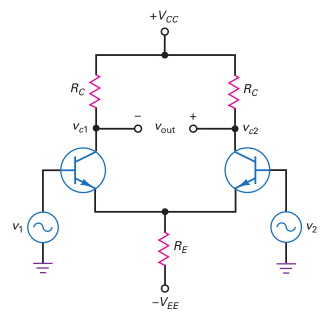
\includegraphics[height=0.7\textheight]{gambar/01.differential_input_output}
		\end{figure}
		\columnbreak
		\begin{itemize}
			\item Ada 2 CE stage yang paralel terhadap resistor \textit{common emitter} $ R_E $
			\item Meskipun ada 2 tegangan \textit{input} ($ v_1 \text{, } v_2$) dan 2 tegangan \textit{collector} ($ v_{c1} \text{, } v_{c2}$), keseluruhan rangkaian dianggap 1 stage.
			\item Tidak ada kapasitor kopling dan bypass $ \rightarrow $ tidak ada lower cutoff frequency
		\end{itemize}
	\end{multicols}
\end{frame}

\begin{frame}{Diferential Input dan Output}
	\begin{multicols}{2}
		\begin{figure}
			\centering
			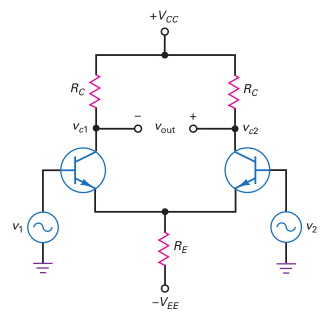
\includegraphics[height=0.7\textheight]{gambar/01.differential_input_output}
		\end{figure}
		\columnbreak
		\begin{itemize}
			\item Tegangan output AC :\\
			
			\begin{equation} \label{pers.1}
				V_{out} =  v_{c2} - v_{c1}
			\end{equation}
		
			\item $ V_{out} $ = differential output, karena menggabungkan 2 tegangan collector.
			\item Transistor yang identik + resistor collector yang sama $ \rightarrow $ ideal
			\item $ v_1 = v_2 \rightarrow v_{out} = 0 $
			\item $ v_1 > v_2 \rightarrow v_{out} $ memiliki polaritas seperti gambar di samping.
			\item $ v_1 < v_2 \rightarrow v_{out} $ inverted + polaritas yang berkebalikan
		\end{itemize}
	\end{multicols}
\end{frame}

\begin{frame}{Diferential Input dan Output}
	\begin{multicols}{2}
		\begin{figure}
			\centering
			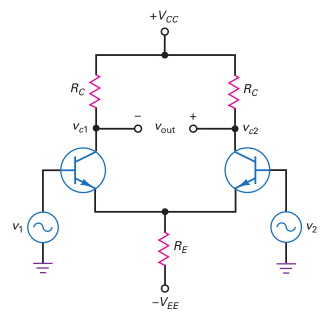
\includegraphics[height=0.7\textheight]{gambar/01.differential_input_output}
		\end{figure}
		\columnbreak
		\begin{itemize}
			\item $ v_1 $ = \textbf{noninverting input} karena $ v_{out} $ memiliki fasa yang sama dengan $ v_1 $
			\item $ v_2 $ = \textbf{inverting input} karena $ v_{out} $ memiliki fasa yang berbeda 180 $ ^{\circ} $ dengan $ v_2 $
			\item Terkadang, noninverting input yang digunakan dan  inverting input di-grounding, terkadang juga sebaliknya.
		\end{itemize}
	\end{multicols}
\end{frame}

\begin{frame}{Diferential Input dan Output}
	\begin{multicols}{2}
		\begin{figure}
			\centering
			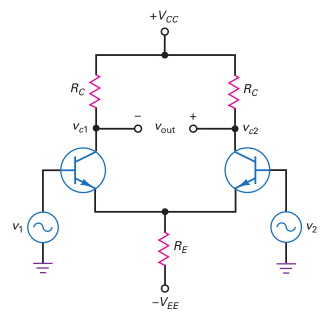
\includegraphics[height=0.7\textheight]{gambar/01.differential_input_output}
		\end{figure}
		\columnbreak
		\begin{itemize}
			\item Jika kedua input-nya ada, input totalnya disebut differential input karena tegangan output sama dengan penguatan tegangan (voltage gain) $ \times $ selisih dari kedua tegangan input.
			\begin{equation} \label{pers.2}
				v_{out} = A_v (v_1 - v_2)
			\end{equation}
			\item $ A_v $ = penguatan tegangan/ voltage gain
		\end{itemize}
	\end{multicols}
\end{frame}

\subsection{Single-Ended Output}
\begin{frame}{Single-Ended Output}
	\begin{multicols}{2}
		\begin{figure}
			\centering
			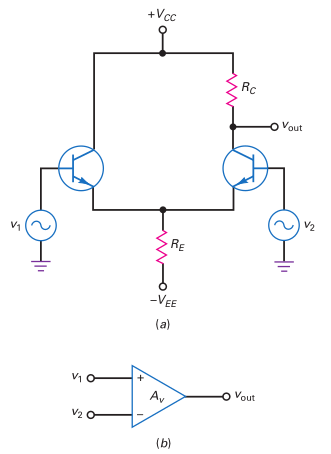
\includegraphics[height=0.8\textheight]{gambar/01.diferential_input_single_ended}
		\end{figure}
		\columnbreak
		\begin{itemize}
			\item Differential output (gambar sebelumnya) membutuhkan floating load, karena kedua ujung dari load tidak ke ground.
			\item Umumnya, load/ beban adalah single-ended, salah satu ujungnya ke ground. Seperti pada gambar (a).
			\item $ V_{out} = A_v (v_1 - v_2) $, tapi voltage gain ($ A_v $) hanya setengah
			\item Blok-diagram, gambar (b), sama dengan op-amp
		\end{itemize}
	\end{multicols}
\end{frame}

\begin{frame}{Konfigurasi Noninverting-Input}
	\begin{multicols}{2}
		\begin{center}
			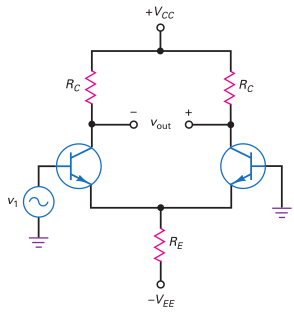
\includegraphics[height=0.7\textheight]{gambar/01.noninverting_input+differential_output}
		\end{center}
		\columnbreak
		\begin{itemize}
			\item Konfigurasi ini memiliki
			\begin{itemize}
				\item Noninverting input
				\item Differential output
			\end{itemize}
			\item Karena $ v_2 = 0 $, maka
		\end{itemize}
		\begin{equation} \label{pers.3}
			v_{out} = A_v (v_1)
		\end{equation}
	\end{multicols}
\end{frame}

\begin{frame}{Konfigurasi Noninverting-Input}
	\begin{multicols}{2}
		\begin{center}
			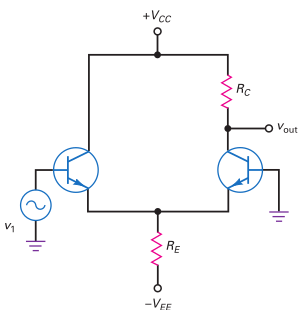
\includegraphics[height=0.7\textheight]{gambar/01.noninverting_input+single-ended_output}
		\end{center}
		\columnbreak
		\begin{itemize}
			\item Konfigurasi ini memiliki
			\begin{itemize}
				\item Noninverting input
				\item Single-ended output
			\end{itemize}
			\item Karena $ v_{out} $ adalah tegangan output AC, maka $ v_{out} $ tetap sama seperti sebelumnya yaitu $ v_{out} = A_v (v_1) $
		\end{itemize}
		\begin{itemize}
			\item Tapi $ A_v $ akan bernilai setengahnya karena output hanya diambil dari satu sisi dari diff-amp
		\end{itemize}
	\end{multicols}
\end{frame}

\subsection{Konfigurasi Inverting-input}
\begin{frame}{Konfigurasi Inverting-input}
	\begin{multicols}{2}
		\begin{center}
			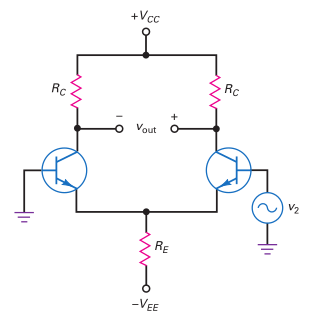
\includegraphics[height=0.7\textheight]{gambar/01.inverting_input+differential_output}
		\end{center}
		\columnbreak
		\begin{itemize}
			\item $ v_2 $ adalah active input dan $ v_1 $ adalah grounded input, maka
			\begin{equation} \label{pers.4}
				v_{out} = -A_v(v_2)
			\end{equation}
			\item Tanda minus (-) menunjukkan fasa yang berkebalikan
		\end{itemize}
	\end{multicols}
\end{frame}

\begin{frame}{Konfigurasi Inverting-input}
	\begin{multicols}{2}
		\begin{center}
			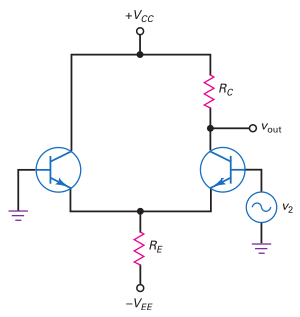
\includegraphics[height=0.7\textheight]{gambar/01.inverting_input+single-ended_output}
		\end{center}
		\columnbreak
		\begin{itemize}
			\item Tegangan output juga sama dengan sebelumnya, yaitu $ v_{out} = -A_v(v_2) $
		\end{itemize}
	\end{multicols}
\end{frame}

\begin{frame}{Ringkasan}
	\begin{center}
		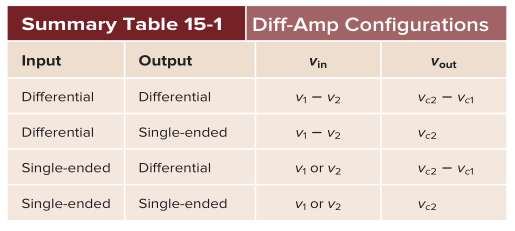
\includegraphics[height=0.6\textheight]{gambar/01.ringkasan_dif-amp-conf}
	\end{center}
\end{frame}

\section{Analisis DC dari Diff Amp}
\begin{frame}{Analisis DC dari Diff Amp}
	\begin{multicols}{2}
		\begin{center}
			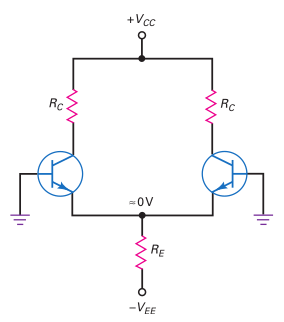
\includegraphics[width=0.7\textheight]{gambar/01.ideal_dc_analysis}
		\end{center}
		\columnbreak
		\begin{itemize}
			\item Rangkaian ekivalen DC dari diff amp.
			\item Pada pembahasan berikutnya, kita akan mengasumsikan transistornya identik dan resistor collectornya sama.
			\item Kita asumsikan juga kedua base di-grounded
		\end{itemize}
	\end{multicols}
\end{frame}

\subsection{Analisis Ideal}
\begin{frame}{Analisis Ideal}
	\begin{multicols}{2}
		\begin{center}
			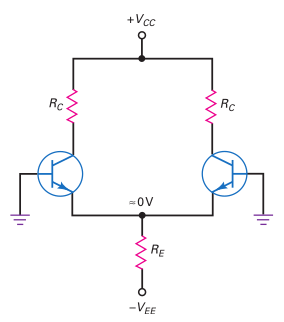
\includegraphics[width=0.7\textheight]{gambar/01.ideal_dc_analysis}
		\end{center}
		\columnbreak
		\begin{itemize}
			\item Diff amp disebut juga long-tail pair karena kedua transistor saling berbagi satu common resistor $ R_E $.
			\item Arus yang mengalir melalui common resistor ini disebut tail current.
			\item Jika kita mengabaikan $ V_{BE} $ drop sepanjang dioda emitter, maka di atas emitter resistor idealnya adalah sebuah titik ground DC.
		\end{itemize}
		\vfill\null
	\end{multicols}
\end{frame}

\begin{frame}{Analisis Ideal}
	\begin{multicols}{2}
		\begin{center}
			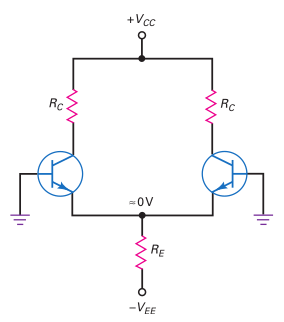
\includegraphics[width=0.7\textheight]{gambar/01.ideal_dc_analysis}
		\end{center}
		\columnbreak
		\begin{itemize}
			\item Sehingga semua $ V_{EE} $ ada di seberang $ R_E $ dan arus tail bernilai
			\begin{equation} \label{pers.5}
				I_T = \frac{V_{EE}}{R_E}
			\end{equation}
			\item Ketika keduanya benar-benar sama, maka arus tail akan terbagi sama, sehingga tiap transistor memiliki arus emitter sebesar \\
			\begin{equation} \label{pers.6}
				I_{EE} = \frac{I_T}{2}
			\end{equation}
		\end{itemize}
		\vfill\null
	\end{multicols}
\end{frame}

\begin{frame}{Analisis Ideal}
	\begin{multicols}{2}
		\begin{center}
			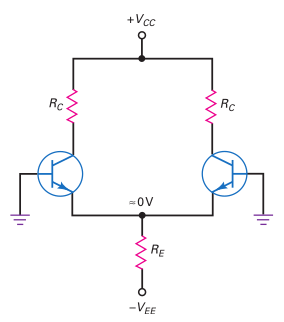
\includegraphics[width=0.7\textheight]{gambar/01.ideal_dc_analysis}
		\end{center}
		\columnbreak
		\begin{itemize}
			\item Tegangan DC pada kedua collector sebesar \\
			\begin{equation} \label{pers.7}
				V_C = V_{CC} - I_C R_C
			\end{equation}
		\end{itemize}
		\vfill\null
	\end{multicols}
\end{frame}

\subsection{Metode kedua}
\begin{frame}{Metode kedua}
	\begin{multicols}{2}
		\begin{center}
			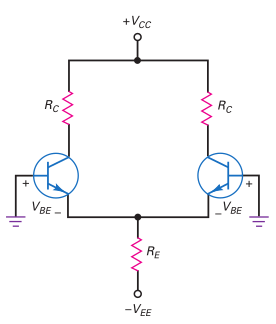
\includegraphics[width=0.7\textheight]{gambar/01.second_approximation}
		\end{center}
		\columnbreak
		\begin{itemize}
			\item Kita bisa meningkatkan analisis DC dengan cara menyertakan $ V_{BE} $ drop di setiap dioda emitter
			\begin{equation} \label{pers.8}
				I_T = \frac{V_{EE} - V_{BE}}{R_E}
			\end{equation}
		\end{itemize}
		\vfill\null
	\end{multicols}
\end{frame}

\subsection{Contoh Soal 1}
\begin{frame}{Contoh Soal 1}
	\begin{multicols}{2}
		\begin{center}
			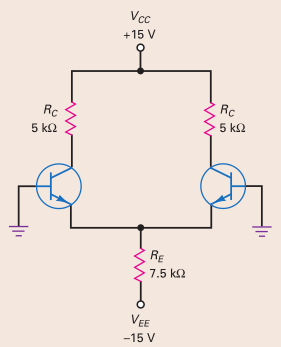
\includegraphics[width=0.6\textheight]{gambar/01.latihan_soal_1a}
		\end{center}
		\columnbreak
		\begin{itemize}
			\item Pertanyaan:
			\begin{itemize}
				\item Berapa arus dan tegangan ideal dari gambar di samping?
			\end{itemize}
			\item Jawaban:
			\begin{itemize}
				\item Berdasarkan persamaan \ref{pers.5}, arus tail adalah:
				\[I_T = \frac{V_{EE}}{R_E} = \frac{15 \text{ v }}{7.5 \text{ m}\Omega} = 2 \text{ mA} \]
				\item Tiap arus emitter adalah separuh dari arus tail:
				\[ I_E = \frac{I_T}{2} = \frac{2 \text{ mA}}{2} = 1 \text{ mA} \]
			\end{itemize}
		\end{itemize}
		\vfill\null
	\end{multicols}
\end{frame}

\begin{frame}{Contoh Soal 1}
	\begin{multicols}{2}
		\begin{center}
			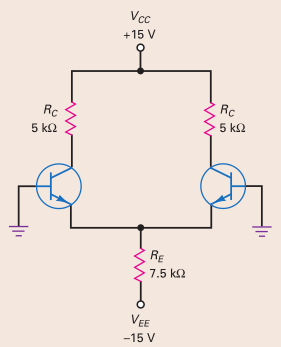
\includegraphics[width=0.6\textheight]{gambar/01.latihan_soal_1a}
		\end{center}
		\columnbreak
		\begin{itemize}
			\item Jawaban:
			\begin{itemize}
				\item Setiap tegangan collectornya adalah:
				\[ V_C = V_{CC} - I_C R_C = 15 \text{ V} - (1 \text{ mA}(5 \text{ k}\Omega)) \]
			\end{itemize}
		\end{itemize}
		\vfill\null
	\end{multicols}
\end{frame}

\section{Referensi}
\begin{frame}{Referensi}
	\begin{enumerate}
		\item test
	\end{enumerate}
\end{frame}

\end{document}

